\documentclass[12pt]{article}
\usepackage[utf8]{inputenc}
\usepackage[russian]{babel}
\usepackage{amsmath,amssymb,amsfonts}
\usepackage{graphicx}
\usepackage{geometry}
\usepackage{hyperref}
\geometry{a4paper,margin=2.5cm}


\usepackage{floatrow,graphicx,calc}
\usepackage{wrapfig}
\usepackage{titlesec}
\usepackage{float}
\usepackage{graphicx}
\graphicspath{{images/}}
\DeclareGraphicsExtensions{.pdf,.png,.jpg}

% --------------------------------------------------
% Макросы для удобства
\newcommand{\rvec}{\mathbf r}
\newcommand{\rone}{\mathbf r_1}
\newcommand{\rtwo}{\mathbf r_2}
\newcommand{\omegav}{\boldsymbol{\omega}}
\newcommand{\muone}{\mu_1}
\newcommand{\mutwo}{\mu_2}
\newcommand{\rh}{\rho}
\newcommand{\dd}{\,\mathrm d}

\title{Устойчивость точек Лагранжа в ограниченной задаче трёх тел\\\small Аналитическое и численное исследование}
\author{}
\date{}

\begin{document}
\maketitle
\tableofcontents
\bigskip

\begin{figure}[H]
  \centering
  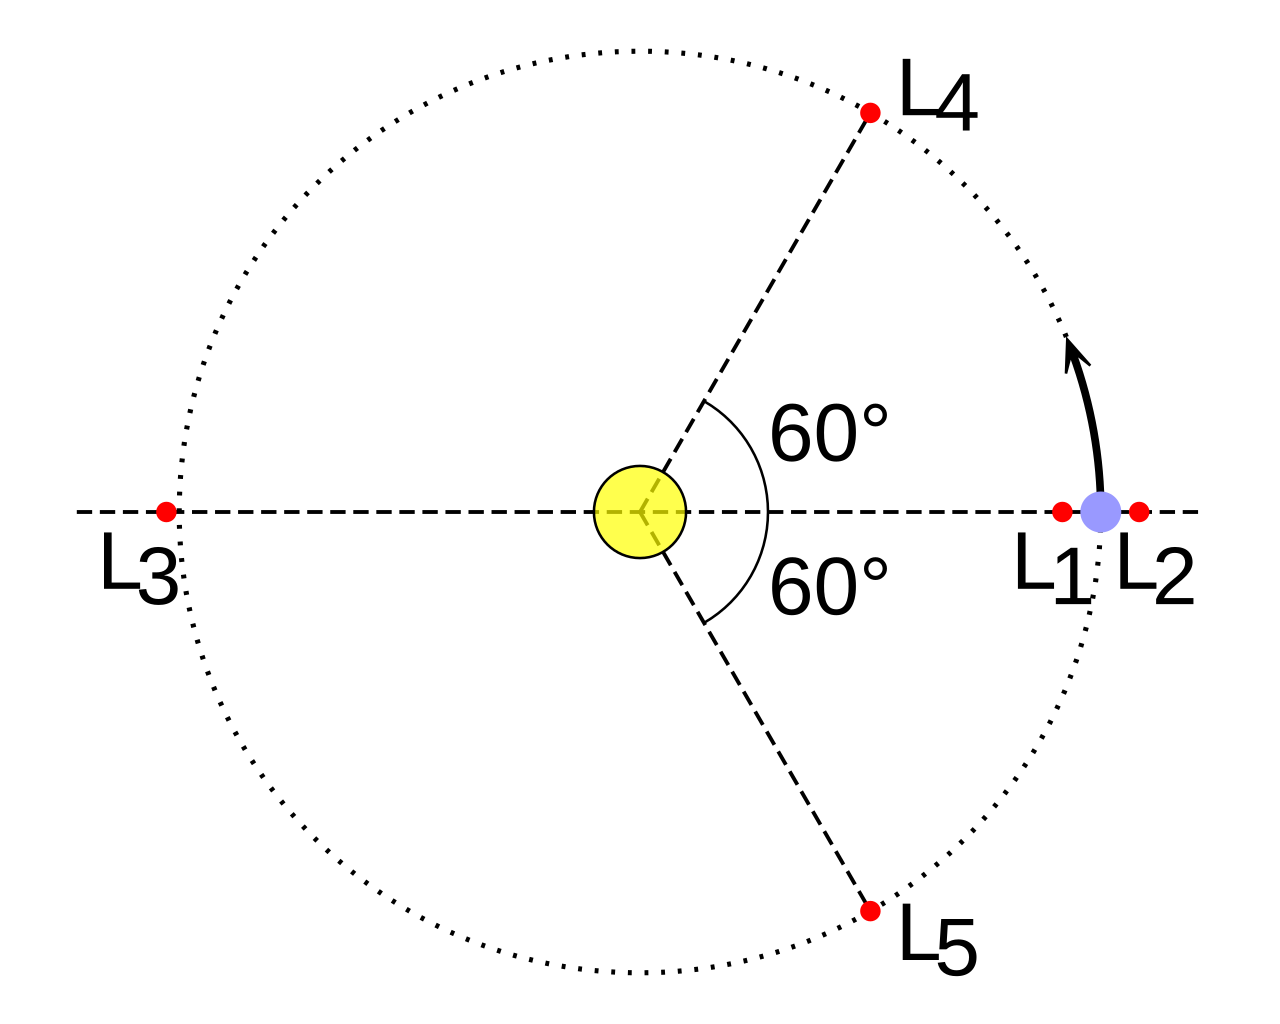
\includegraphics[width=0.6\textwidth]{image.png}
  \caption{Положения точек Лагранжа}
  \label{fig:lagr}
\end{figure}

% ==================================================
\section{Со‑вращающаяся система отсчёта}\label{sec:corot}

Перейдём к неинерциальной системе координат, вращающейся с постоянной угловой скоростью $\omega$ вокруг оси, перпендикулярной плоскости орбит масс $m_1$ и $m_2$ и проходящей через их центр масс. В такой со‑вращающейся системе $m_1$ и $m_2$ покоятся. Введём декартову систему координат $(x,y)$ так, чтобы обе массивные частицы всегда находились на оси~$x$.

Массы $m_1$ и $m_2$ занимают фиксированные положения
\begin{equation}\label{eq:r1r2}
  \rone = \mutwo\,(-1,0,0),\qquad
  \rtwo = \muone\,(1,0,0),
\end{equation}
где $\mu_1=m_1/(m_1+m_2)$ и $\mu_2=m_2/(m_1+m_2)$, а положение пробной массы $m_3$ опишем вектором. 

Можно также ввести общий коэффициент $ \mu=m_2/(m_1+m_2) \quad \mu_2 = \mu, \mu_1 = 1 - \mu$, использовался в численных методах

\begin{equation}\label{eq:rvec}
  \rvec = (x,y,z).
\end{equation}

\begin{figure}[H]
  \centering
  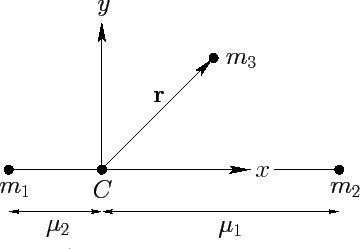
\includegraphics[width=0.55\textwidth]{image1.png}
  \caption{Со‑вращающаяся система координат, связанная с массами $m_1$ и $m_2$.}
  \label{fig:corot}
\end{figure}

Уравнение движения $m_3$ в этой системе имеет вид
\begin{equation}\tag{1050}\label{eq:1050}
  \ddot{\rvec}+2\omegav\times\dot{\rvec}
  = -\frac{\muone\,(\rvec-\rone)}{\rho_1^{3}}
    -\frac{\mutwo\,(\rvec-\rtwo)}{\rho_2^{3}}
    +\omegav\times(\omegav\times \rvec),
\end{equation}
где $\omegav=(0,0,\omega)$, а
\begin{align}\tag{1051}\label{eq:rho1}
  \rho_1^{2} &= (x+\mutwo)^2 + y^{2}+z^{2},\\[2pt]
  \rho_2^{2} &= (x-\muone)^2 + y^{2}+z^{2}.\tag{1052}\label{eq:rho2}
\end{align}
Второй член в левой части~\eqref{eq:1050} — кориолисово ускорение, а последний член в правой части — центробежное ускорение.

Рассматривая декартовы компоненты, из~\eqref{eq:1050} получаем
\begin{align}\tag{1053}\label{eq:1053}
  \ddot x - 2\omega\dot y &= -\frac{\muone\,(x+\mutwo)}{\rho_1^{3}}-\frac{\mutwo\,(x-\muone)}{\rho_2^{3}}+\omega^{2}x,\\[2pt]
\tag{1054}\label{eq:1054}
  \ddot y + 2\omega\dot x &= -\biggl(\frac{\muone}{\rho_1^{3}}+\frac{\mutwo}{\rho_2^{3}}\biggr)y + \omega^{2}y,\\[2pt]
\tag{1055}\label{eq:1055}
  \ddot z &= -\biggl(\frac{\muone}{\rho_1^{3}}+\frac{\mutwo}{\rho_2^{3}}\biggr)z.
\end{align}

Введём комбинированный потенциал (гравитационный $+$ центробежный)
\begin{equation}\tag{1059}\label{eq:U}
  U(x,y,z) = -\frac{\muone}{\rho_1}-\frac{\mutwo}{\rho_2}-\frac{\omega^{2}}{2}(x^{2}+y^{2}).
\end{equation}
Тогда уравнения\,(\ref{eq:1053})–(\ref{eq:1055}) можно записать компактно как
\begin{equation}\tag{1056--1058}
  \ddot {\mathbf q} + 2\omegav\times\dot{\mathbf q} = -\nabla U,\qquad \mathbf q=(x,y,z).
\end{equation}
Следует дифференциальное тождество
\begin{equation}\tag{1063}\label{eq:jacobi}
  \frac{\dd}{\dd t}\Bigl[\tfrac12(\dot x^{2}+\dot y^{2}+\dot z^{2})+U\Bigr]=0,
\end{equation}
что приводит к интегралу Якоби
\begin{equation}\tag{1064}
  C = -2U-v^{2},\qquad v^{2}=\dot x^{2}+\dot y^{2}+\dot z^{2},
\end{equation}
ограничивающему область допустимого движения условием $-2U\ge C$. \par
\bigskip

% ==================================================
\section{Устойчивость точек Лагранжа}\label{sec:stability}

Пять точек Лагранжа~$L_1$–$L_5$ являются точками равновесия для массы $m_3$ в со‑вращающейся системе. Определим их устойчивость при малых возмущениях.

\subsection{Движение в плоскости $xy$}
Пусть координаты точки Лагранжа $(x_0,y_0,0)$. Для малых отклонений положим
\begin{equation}\tag{1097--1099}
  x=x_0+\delta x,\qquad y=y_0+\delta y,\qquad z=0.
\end{equation}
Разложив потенциал в ряд Тейлора до второго порядка и учитывая, что $\nabla U=0$ в самой точке, получим
\begin{equation}\tag{1101}\label{eq:Uxy}
  U\approx U_0+\tfrac12 U_{xx}\,\delta x^{2}+U_{xy}\,\delta x\,\delta y+\tfrac12 U_{yy}\,\delta y^{2}.
\end{equation}
Подставляя~\eqref{eq:Uxy} в линеризованные уравнения движения и полагая $\delta x,\delta y\propto e^{\gamma t}$, приходим к системе
\begin{align}\tag{1104}\label{eq:matrix}
  \begin{pmatrix}
    \gamma^{2}+U_{xx} & -2\gamma+U_{xy}\\[4pt]
    2\gamma+U_{xy} & \gamma^{2}+U_{yy}
  \end{pmatrix}
  \begin{pmatrix}\delta x_0\\ \delta y_0\end{pmatrix}=\begin{pmatrix}0\\0\end{pmatrix}.
\end{align}
Необходимое условие ненулевого решения — зануление детерминанта, что даёт уравнение
\begin{equation}\tag{1105}\label{eq:quartic}
  \gamma^{4}+(4+U_{xx}+U_{yy})\gamma^{2}+(U_{xx}U_{yy}-U_{xy}^{2})=0.
\end{equation}

Введём обозначения
\begin{align}\tag{1106--1109}
  A &= \frac{\muone}{\rho_1^{3}}+\frac{\mutwo}{\rho_2^{3}}, &
  B &= 3\bigl(\frac{\muone}{\rho_1^{5}}+\frac{\mutwo}{\rho_2^{5}}\bigr)y^{2},\\
  C &= 3\bigl[\frac{\muone(x+\mutwo)}{\rho_1^{5}}+\frac{\mutwo(x-\muone)}{\rho_2^{5}}\bigr]y, &
  D &= 3\bigl[\frac{\muone(x+\mutwo)^{2}}{\rho_1^{3}}+\frac{\mutwo(x-\muone)^{2}}{\rho_2^{3}}\bigr],
\end{align}
что приводит к
\begin{equation}\tag{1110--1112}
  U_{xx}=A-D-1,\quad U_{yy}=A-B-1,\quad U_{xy}=-C.
\end{equation}

\subsubsection{Коллинеарные точки $L_1,\,L_2,\,L_3$}
Для $y=0$ получаем $B=C=0$, $D=3A$, откуда
\begin{equation}\label{eq:Ucol}\tag{*}
  U_{xx}=-1-2A,\quad U_{yy}=A-1,\quad U_{xy}=0.
\end{equation}
Обозначив $\Gamma=\gamma^{2}$, характеристическое уравнение принимает вид
\begin{equation}\tag{1113}
  \Gamma^{2}+(2-A)\Gamma+(1-A)(1+2A)=0.
\end{equation}
Обозначим
\[
a_1=2-A,\qquad a_0=(1-A)(1+2A).
\]
Для действительных корней справедливо(т.Виета)
\[
\Gamma_1+\Gamma_2=-a_1=-(2-A),\qquad \Gamma_1\Gamma_2=a_0.
\]
Чтобы оба корня были \emph{отрицательными}, необходимо и достаточно
\[
\Gamma_1+\Gamma_2<0\;(\text{сумма отрицательна}),\qquad \Gamma_1\Gamma_2>0\;(\text{произведение положительно}).
\]
Откуда
\begin{align}
&-(2-A)<0\;\Longrightarrow\;2-A>0\;\Longrightarrow\;A<2,\\[4pt]
&(1-A)(1+2A)>0.
\end{align}
Поскольку \(1+2A>0\) при всех \(A>-\tfrac12\), второе неравенство эквивалентно
\[ A<1. \]
Требование вещественности (дискриминант):
\begin{equation}
D=(2-A)^2-4(1-A)(1+2A)=9A^{2}-8A=A\bigl(9A-8\bigr)\ge0.
\end{equation}
При условии \(A>0\) получаем 
\[ A\ge\frac89. \]
Сводя воедино требования
\[ A<1,\quad A\ge\frac89, \]
получаем 
\begin{equation}
\frac89\le A<1
\end{equation}


Используя условие на дискриминант и т.Виета получаем, что корни будут отрицательными и действительными лишь при
\begin{equation}\tag{1115}
  \frac{8}{9}\le A\le1.
\end{equation}
На рис.~\ref{fig:A_vs_mu} показано, что для любых $0<\mutwo\le0.5$ величина $A$ в точках $L_1$–$L_3$ превышает 1, значит, везде $\exists\lambda:Re\lambda > 0$, поэтому эти точки неустойчивы.

\begin{figure}[H]
  \centering
  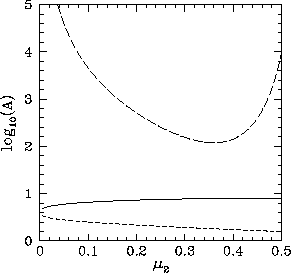
\includegraphics[width=0.6\textwidth]{image2.png}
  \caption{Зависимость параметра $A$ от массового отношения $\mutwo$ для коллинеарных точек $L_1$, $L_2$ и $L_3$.}
  \label{fig:A_vs_mu}
\end{figure}

\subsubsection{Треугольные точки $L_4$ и $L_5$}
Для этих точек $\rho_1=\rho_2=1$, откуда $A=1$, $B=9/4$, $D=3/4$ и
\[U_{xy}=\mp\sqrt{27/16}\,(1-2\mutwo).\]
Уравнение на $\Gamma$:
\begin{equation}\tag{1116}
  \Gamma^{2}+\Gamma+\frac{27}{4}\,\mutwo(1-\mutwo)=0.
\end{equation}
Чтобы корни были также действительными, проверяем дискриминант:
\begin{equation}
D=1-4a_0=1-27\,\mu_2\bigl(1-\mu_2\bigr)\ge0.
\end{equation}
Преобразуем:
\begin{align}
1-27\mu_2+27\mu_2^2&\ge0,\\[2pt]
27\mu_2^2-27\mu_2+1&\ge0.
\end{align}
Это квадратное неравенство имеет корни
\[\mu_{\pm}=\frac12\Bigl(1\pm\sqrt{\frac{23}{27}}\Bigr).
\]
Поскольку рассматриваемый физический параметр удовлетворяет \(0<\mu_2<1\),
из двух интервалов
\(\bigl(-\infty,\mu_-\bigr]\cup\bigl[\mu_+,\infty\bigr)\)
нас интересует лишь левый.  Следовательно,
\begin{equation}\tag{1117}
  \mutwo<\frac12\bigl(1-\sqrt{23/27}\bigr)\approx0.0385.
\end{equation}
Обозначив за критическое значение удельной массы $\mu_{crit} = \frac12\bigl(1-\sqrt{23/27}\bigr)\approx0.0385$
\begin{equation}\tag{1118}
  \mu = \frac{m_2}{m_1+m_2}< \mu_{crit}.
\end{equation}

Если малое тело удовлетворяет этому условию, возмущённое движение вокруг $L_4$ или $L_5$ остаётся ограниченным, что подтверждается орбитами троянских астероидов Юпитера и пылевыми облаками в системе Солнце–Земля.

Возвращаясь к ~\eqref{eq:1050} получаем, что $a_1(\text{при }\gamma^3) = 0,\quad a_3(\text{при }\gamma) = 0$ и условие, если $\mutwo < 0.0385$, то $\forall Re\lambda_i \leqslant 0$ - устойчивы по Ляпунову. При $\mutwo \geqslant 0.0385$ будет $\exists\lambda: Re\lambda > 0$, значит - неусточивые.

\bigskip

\subsection{Итоги аналитического метода}

Для 5 точек лагранжа: 
\begin{itemize}
    \item Коллинеарные точки $L_1,L_2,L_3$ - неустойчивы по Ляпунову$\forall \mu$
    \item Треугольные точки $L_4, L_5$ - устойчивы по Ляпунову при $\mu<\mu_{crit}$ и неустойчивы при $\mu \geqslant \mu_{crit}$
\end{itemize}

\section{Моделирование точек Лагранжа}\label{sec:model}

Инетгрированием уравнений движения и строя графики зависимости, исследуем устойчивость

Используя $m_1=1,\Omega = 1, R=1, t = 100$ и имея один параметр $\mu(m_1=1,m_2) = \mu(m_2)$ рассмотрим график траекторий, фазового портрета, а также расстояния до точки Лагранжа от времени, сделаем выводы.

Будем рассматривать $L_1,L_4$:

\subsection{$\mu=0.03$}

\begin{figure}[H]
  \centering
  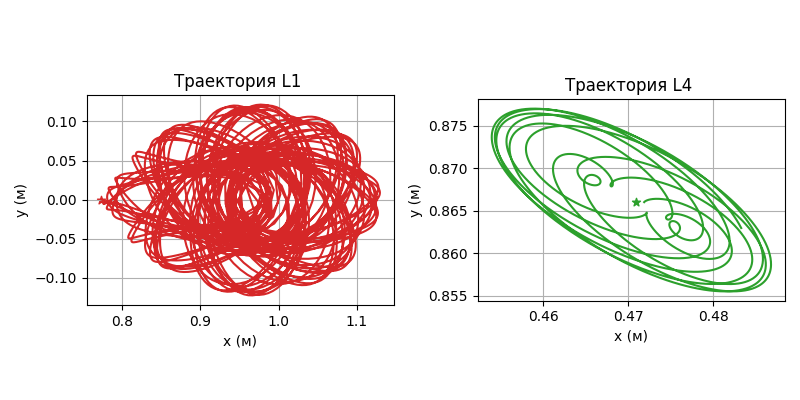
\includegraphics[width=1\textwidth]{Figure_1.png}
  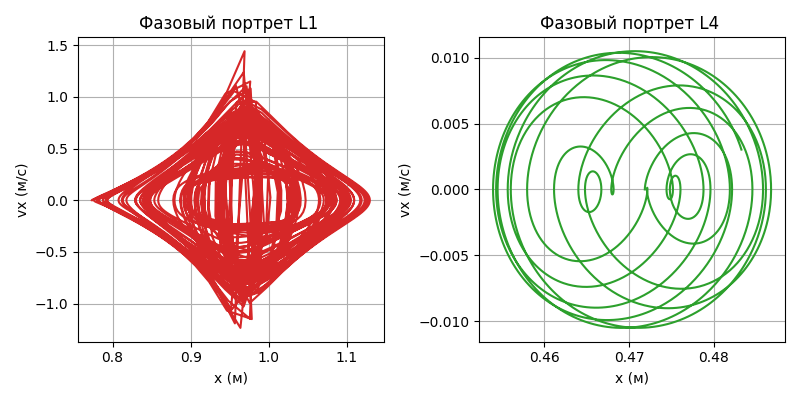
\includegraphics[width=1\textwidth]{Figure_2.png}
  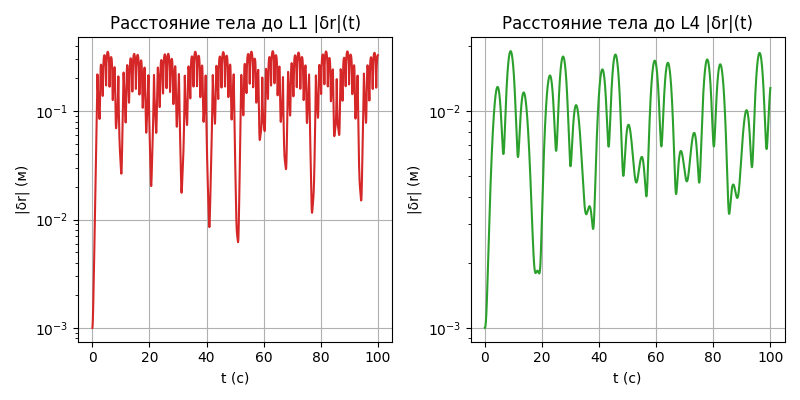
\includegraphics[width=1\textwidth]{Figure_3.png}
\end{figure}

\begin{itemize}
  \item \textbf{Параметры модели:} $m_1=1$, $m_2=0.03\quad(\mu=0.0291<0.03852)$.
  \item \textbf{Графики траекторий $(x,y)$:}\\
        для $L_4$ -- узкая замкнутая кривая;\\
        для $L_1$ -- расходящаяся спираль. 
  \item \textbf{Фазовые портреты $(x,v_x)$:}\\
        для $L_4$ даёт концентрические овалы (центр Ляпунова);\\
        для $L_1$ заполняет ромбическую область (седло).
  \item \textbf{Лог‑графики расстояния $|\delta r|(t)$:}\\
        $L_4$: амплитуда остаётся в пределах $10^{-3}$--$10^{-2}$~м;\\
        $L_1$: быстро растёт до $\sim10^{-1}$~м, далее колеблется возле потолка.
\end{itemize}

\subsection{$\mu=0.047$} 

\begin{figure}[H]
  \centering
  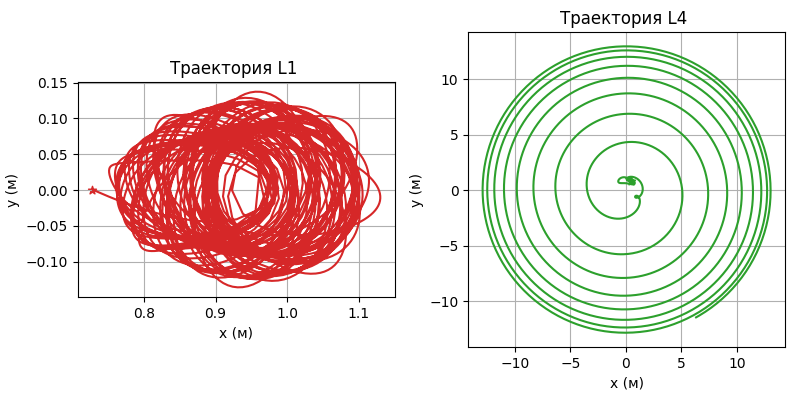
\includegraphics[width=1\textwidth]{Figure_11.png}
  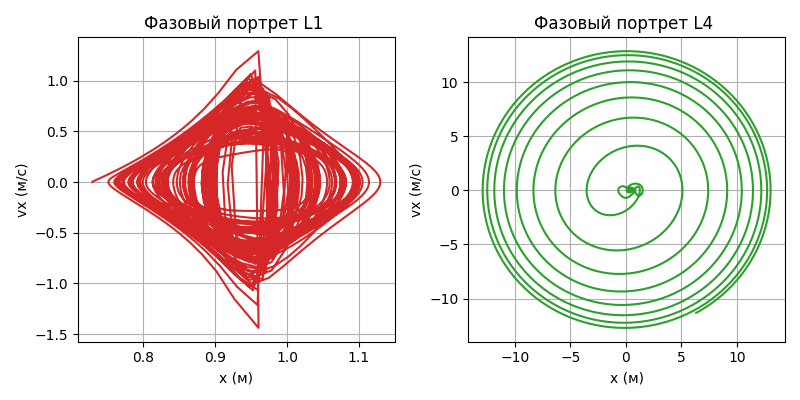
\includegraphics[width=1\textwidth]{Figure_22.png}
  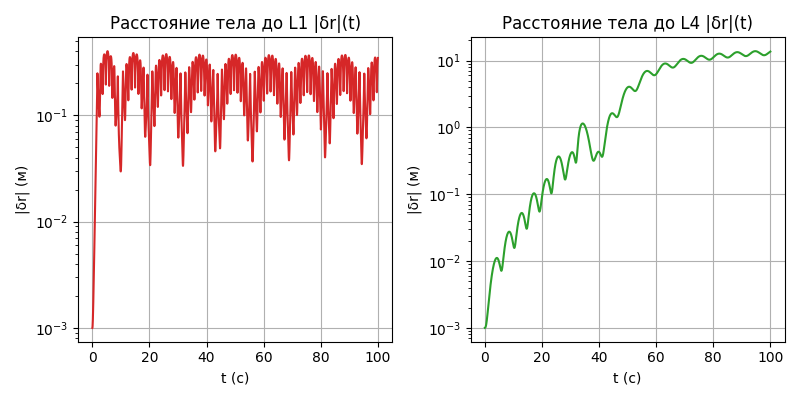
\includegraphics[width=1\textwidth]{Figure_33.png}
\end{figure}

\begin{itemize}
  \item \textbf{Параметры модели:} $m_1=1$, $m_2=0.047\quad(\mu=0.044>0.03852)$.
  \item \textbf{Графики траекторий $(x,y)$:}\\
        для $L_4$ -- расходящаяся спираль;\\
        для $L_1$ -- расходящаяся спираль. 
  \item \textbf{Фазовые портреты $(x,v_x)$:}\\
        для $L_4$ расходящаяся окружность;\\
        для $L_1$ расходящийся ромб(седло).
  \item \textbf{Лог‑графики расстояния $|\delta r|(t)$:}\\
        $L_4$:  Наличие вещественного положительного собственного значения $\lambda$. Тело удаляется от точки Лагранжа;\\
        $L_1$: Виден рост расстояния от точки Лагранжа и достижение барьера ПНС.
\end{itemize}

\subsection{$\mu=0.057$} 

\begin{figure}[H]
  \centering
  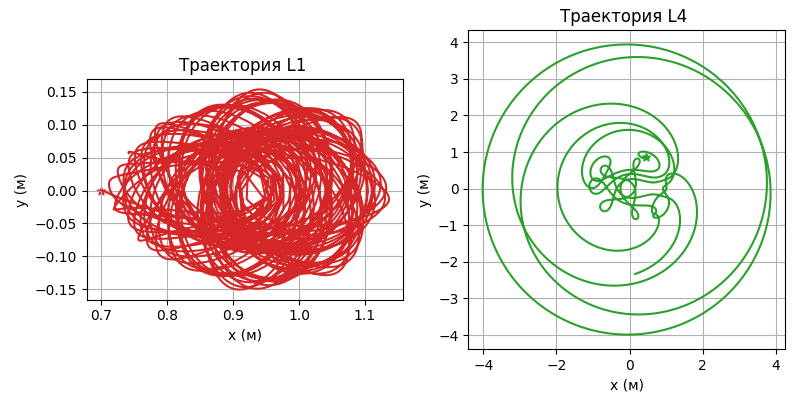
\includegraphics[width=1\textwidth]{Figure_111.png}
  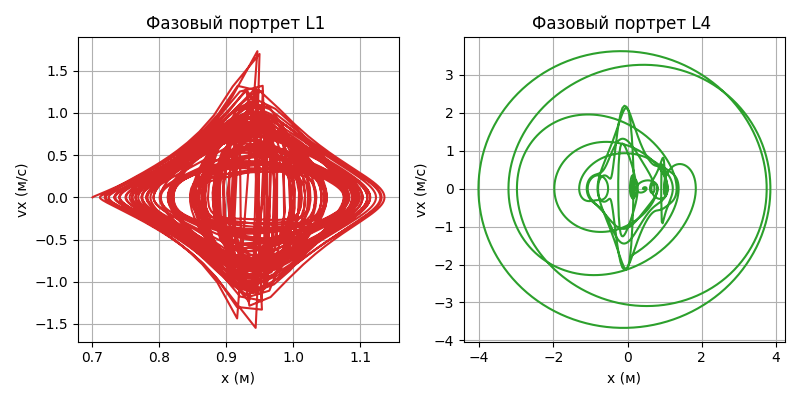
\includegraphics[width=1\textwidth]{Figure_222.png}
  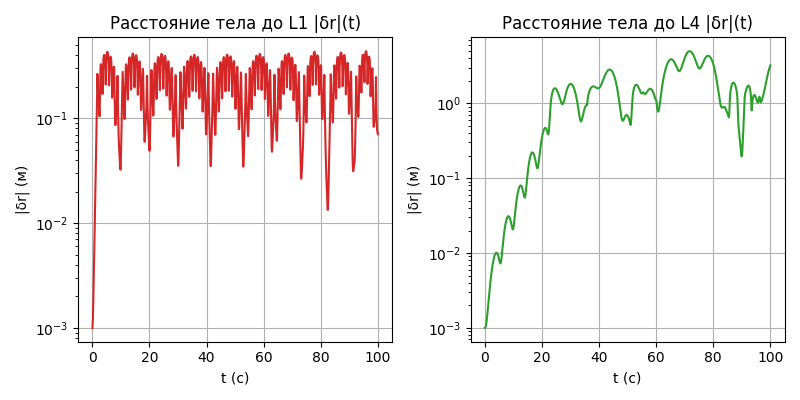
\includegraphics[width=1\textwidth]{Figure_333.png}
\end{figure}

\begin{itemize}
  \item \textbf{Параметры модели:} $m_1=1$, $m_2=0.06\quad(\mu=0.057>0.03852)$.
  \item \textbf{Графики траекторий $(x,y)$:}\\
        для $L_4$ -- смещение центра фигуры в $m_1$ - уход из точки Лагранжа;\\
        для $L_1$ -- расходящаяся спираль. 
  \item \textbf{Фазовые портреты $(x,v_x)$:}\\
        для $L_4$ расходящаяся окружность с начальным ромбом;\\
        для $L_1$ расходящийся ромб(седло).
  \item \textbf{Лог‑графики расстояния $|\delta r|(t)$:}\\
        $L_4$:  Наличие вещественного положительного собственного значения $\lambda$. Тело удаляется от точки Лагранжа;\\
        $L_1$: Виден рост расстояния от точки Лагранжа и достижение барьера ПНС.
\end{itemize}



\subsection{Интеграл Якоби}

В плоской ограниченной круговой задаче трёх тел действует первый интеграл
\[
C \;=\; 2\,U_{\mathrm{эфф}}(x,y)\;-\;\bigl(\dot x^{2}+\dot y^{2}\bigr)
\quad(\text{постоянен по времени}),
\]
где
\(
U_{\mathrm{эфф}} = -\frac{1-\mu}{r_1}-\frac{\mu}{r_2}-\tfrac12(x^{2}+y^{2})
\)
— эффективный потенциал во вращающейся системе.

Из него следует \emph{неравенство нулевой скорости}
\[
\dot x^{2}+\dot y^{2}=2U_{\mathrm{эфф}}-C \;\;\Longrightarrow\;\;
2U_{\mathrm{эфф}}(x,y)\;\ge\;C .
\]
Области, где $2U_{\mathrm{эфф}}<C$, \emph{запрещены} для движения
(пришлось бы иметь отрицательную кинетическую энергию).

Поверхность $2U_{\mathrm{эфф}}=C$ называют \textbf{поверхностью нулевой скорости} (ПНC);

\subsection*{2. Критические уровни $C_i$}

Для каждой точки Лагранжа
\[
C_i = 2\,U_{\mathrm{эфф}}(L_i).
\]

\begin{itemize}
  \item $L_1,L_2,L_3$ --- \emph{седловые} точки $U_{\mathrm{эфф}}$: \
        ПНC имеет ``горловины'' (necks), которые открываются/закрываются
        в зависимости от того, выше или ниже текущий $C$ относительного $C_i$.
  \item $L_4,L_5$ --- \emph{минимумы} $U_{\mathrm{эфф}}$: \
        окрестность точки всегда лежит {\it внутри} допускаемой области,
        а вокруг имеется замкнутый ``остров'' уровня $C$.
\end{itemize}

\section{Источники}

\url{https://ru.wikipedia.org/wiki/Задача_трёх_тел}\\
\url{https://ru.wikipedia.org/wiki/Интеграл_Якоби}\\
\url{https://ocw.mit.edu/courses/aeronautics-and-astronautics/16-07-dynamics-fall-2009/lecture-notes/MIT16_07F09_Lec18.pdf}\\
\url{https://farside.ph.utexas.edu/teaching/336k/Newton/node124.html}\\
\url{https://farside.ph.utexas.edu/teaching/336k/Newton/node126.html}\\
\url{https://math-mech-astr-journal.spbu.ru/article/view/15502/10422}\\

\end{document}
